\chapter{Architecture}

This section discusses the architecture of libbind \todo{lib needs renaming} and presents its constituent components. The actual implementation will be covered separately so there may be minor inaccuracies and inconsistencies to keep things simple. Particularly, one key aspect of the library that should be noted is the support for both x86-32 and x86-64. While there is a high degree of overlap in code dealing with these architectures, the library delegates the work to architecture-specific sub-components for certain tasks such as instruction manipulation. Such differences will be addressed in Implementation\todo{make ref}, but ignored for now.

The following diagram illustrates the three main components of libbind:

\begin{figure}[H]
 \centering
 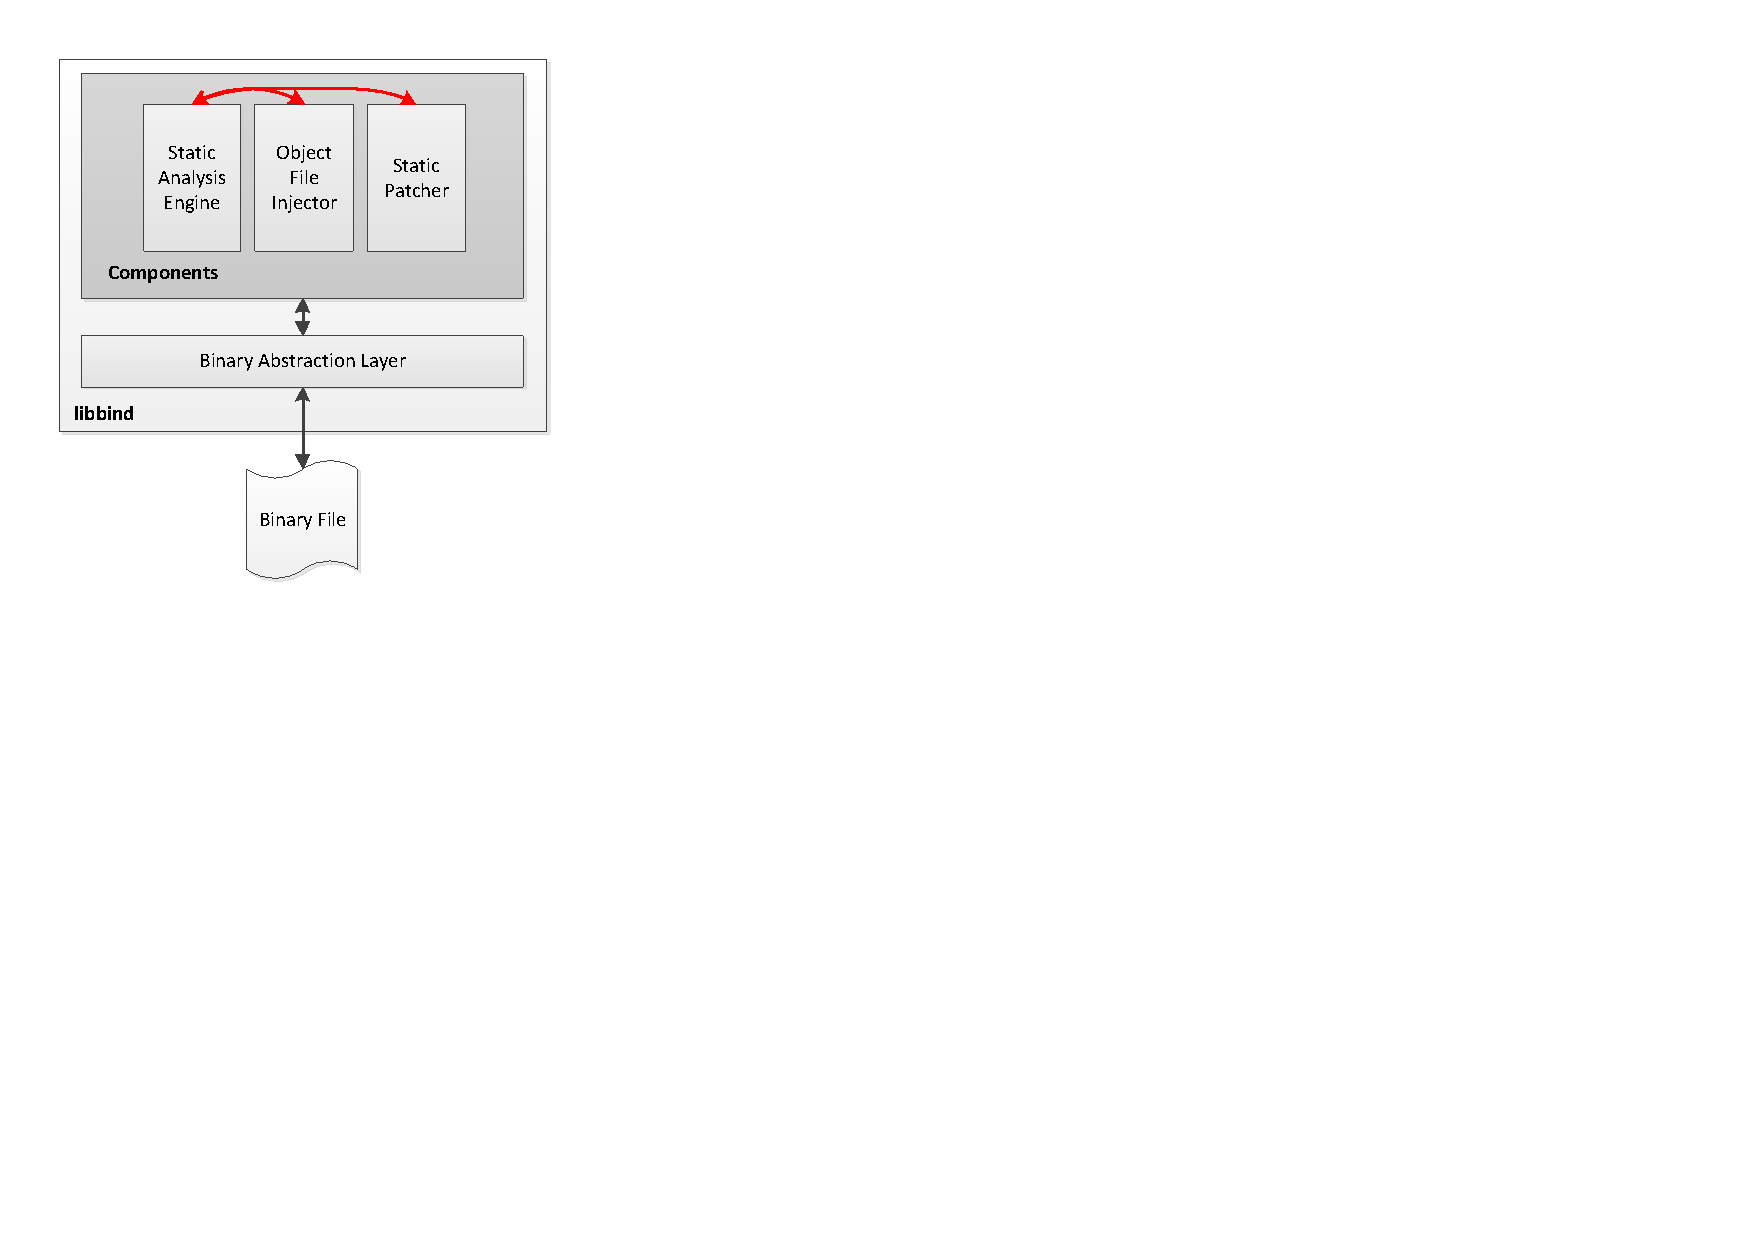
\includegraphics{Architecture.pdf}
 \caption[Architecture]{The high level architecture of libbind. The three components of libbind interact with a binary file through an internal binary abstraction layer. Within the library, the static analysis engine collaborates with the object file injector and static patcher.}
\end{figure}

The choice for the different components of libbind is mainly due to the natural and inherent separation in duty between the three aspects. The components interact through a well-defined interface which means the implementations are fully decoupled. This allows different implementations to be 'plugged in' increasing the portability value of the library. For example, it is trivial to write a static analysis engine plugin for a different architecture as long as the new implementation adheres to the original interface.

For now, we can treat the binary abstraction layer as libbind's internal representation of a binary file. Most importantly, the binary abstraction layer encapsulates the internal representation of the code of a binary as a CFG as required by \emph{(F4)} and \emph{(F5)} of the specification. As such, any modifications to the code of a binary are done through the addition, deletion or modification of nodes/vertices in the CFG. Hence, a simplified and abstract way of considering each component of libbind is in terms of the operations it performs upon the CFG.

\section{Static Analysis Engine}

\begin{figure}[H]
 \centering
 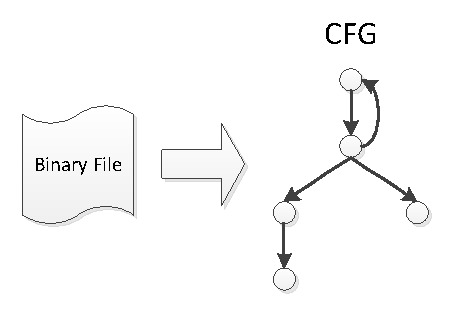
\includegraphics{Static_Analysis_Engine.pdf}
 \caption[Static Analysis Engine]{The primary role of the static analysis engine is to \emph{generate a CFG}.}
\end{figure}

While the fundamental goal of libbind is to provide static detouring, the usefulness of such a feature is greatly diminished without the appropriate supporting functionality. If a user were required to provide raw addresses to patch, it would not be feasible to use the library standalone. The static analysis engine essentially plays a supporting role which can be split into three parts:

\begin{description}
\item[Disassembler Engine] This is required for the construction of the CFG. The sole purpose of the disassembler engine is to perform the heavy lifting in terms of mapping the raw bytes of a binary to useful semantic information. For example, given an arbitrary address, the disassembler engine can disassemble the instruction held at that address and determine whether that instruction is a branching one and if so, decode the operand and attempt to figure out the branch destination.
\item[CFG Analysis] The generation of a CFG starts by pointing the disassembler engine to a root of disassembly (such as the entry point). Using the information provided by the disassembler engine, the analysis uses an algorithm to perform a depth-first discovery of the program structure.
\item[Symbol Table Parser] A symbol table is not guaranteed to exist in a binary because it can be completely stripped during or after compilation. The symbol table parser checks for the existence of a symbol table and if found stores the symbol information alongside the CFG.
\end{description}

To summarise, there are two phases to the static analysis performed by libbind. Firstly, a CFG is generated and then in the second pass, symbol information is added to the CFG. The CFG exposes an access interface through which a user is able to locate and express the source and destination for static patching. This is a concrete example of how the presence of a symbol table is beneficial. If we first consider a CFG without symbol information, the only way of identifying a basic block or function is to specify a heuristic in terms of instructions and iterate all basic blocks till a match is found. For example:

\noindent\begin{minipage}{\textwidth}
\begin{lstlisting}[language=C,caption={Identifying basic blocks via instruction heuristics}]
/*
 * Checks whether the first instruction is "push %rbp"
 */
struct bf_basic_blk * bb;

bf_for_each_basic_blk(bb, bf) {
  if(bb->insn_vec[0]->mnemonic == push_insn &&
      bb->insn_vec[0]->operand1->tag == OP_REG &&
      bb->insn_vec[0]->operand1->operand_info->reg == rbp_reg &&
      ...) {
    bf_trampoline_basic_blk(bf, bb, dest_bb);
    break;
  }
}
\end{lstlisting}
\end{minipage}

Basic block (and function) identification through instruction heuristics is verbose but necessary in order to be able to search at an instruction granularity. If available, a symbol table is a valuable resource that allows a far more convenient method of locating the same basic blocks/functions. Assuming the basic block we are searching for is actually the first basic block of a function named \emph{func1}, the identification could be expressed alternatively:

\begin{lstlisting}[language=C,caption={Identifying basic blocks via symbols}]
/*
 * Locates a function by its name.
 */
struct bf_func * func = symbol_find(&bf->sym_table, "func1");
bf_trampoline_func(bf, func, dest_func);
\end{lstlisting}

The functionality provided by the static analysis engine is powerful and can be used in many other applications. For example, it is possible to compare the CFG of two binaries to generate statistics for the number of changed functions/basic blocks/instructions. This is not a feature that is provided directly by libbind because it aims to be a general purpose library. It is a specific application of the static analysis engine and we demonstrate this as part of our evaluation.

\section{Object File Injector}

\begin{figure}[H]
 \centering
 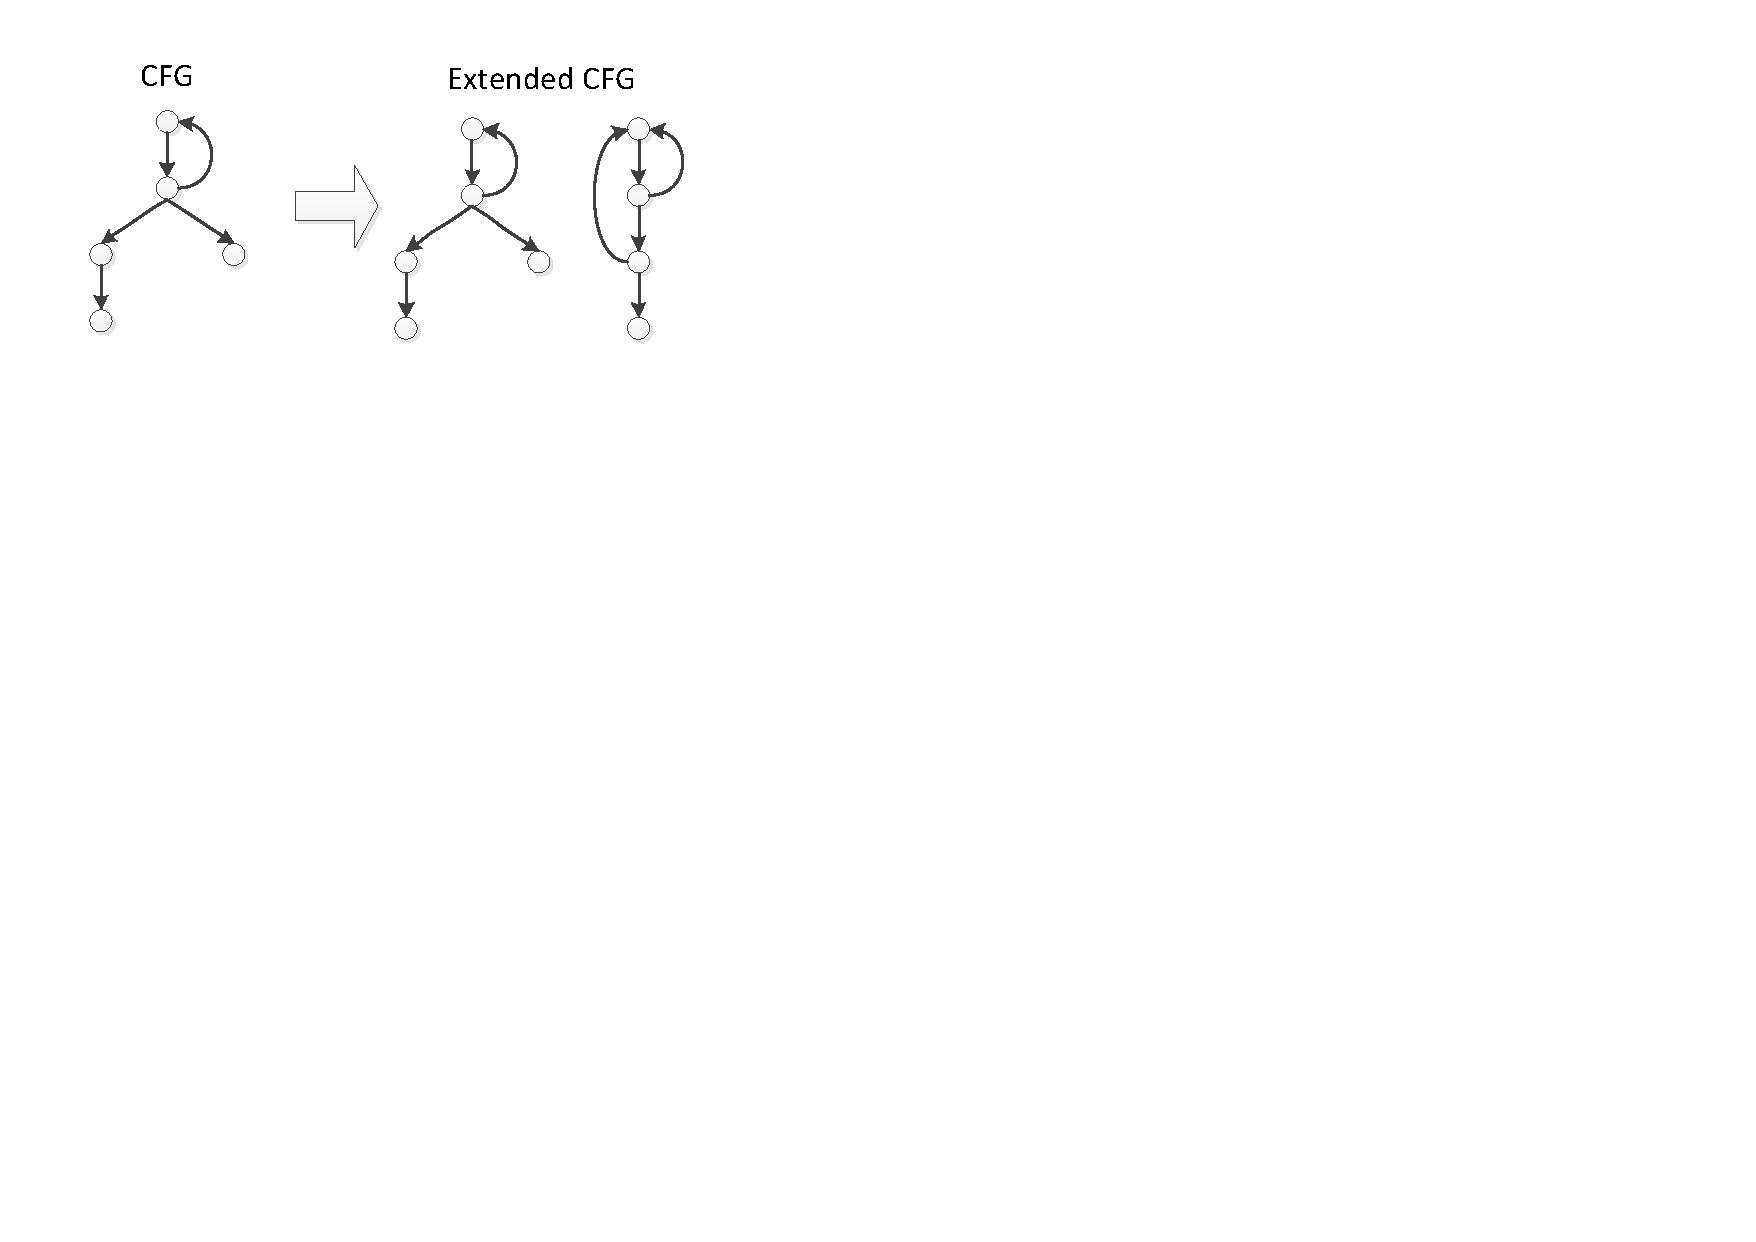
\includegraphics{Object_File_Injector.pdf}
 \caption[Object File Injector]{The role of the object file injector is to extend the CFG such that the CFG after injection is a superset of the CFG before injection. That is, a set of \emph{nodes and edges are added} which are disjoint to the original CFG.}
\end{figure}

The function of the object file injector is to load extra code into the target binary. Immediately after injection, the new code is unreachable from the original code which explains the two disjoint parts of the resulting CFG. The implication is that the injected CFG can be hooked up with the original CFG via the static patcher. Trampolining from the original code to the new code and back allows the semantics of target to be extended while preserving existing functionality.

The ability to load external code into the target binary is necessary in order to instrument the code at all. However, object file injection is a highly non-trivial process as we will see in later sections.

\section{Static Patcher}

\begin{figure}[H]
 \centering
 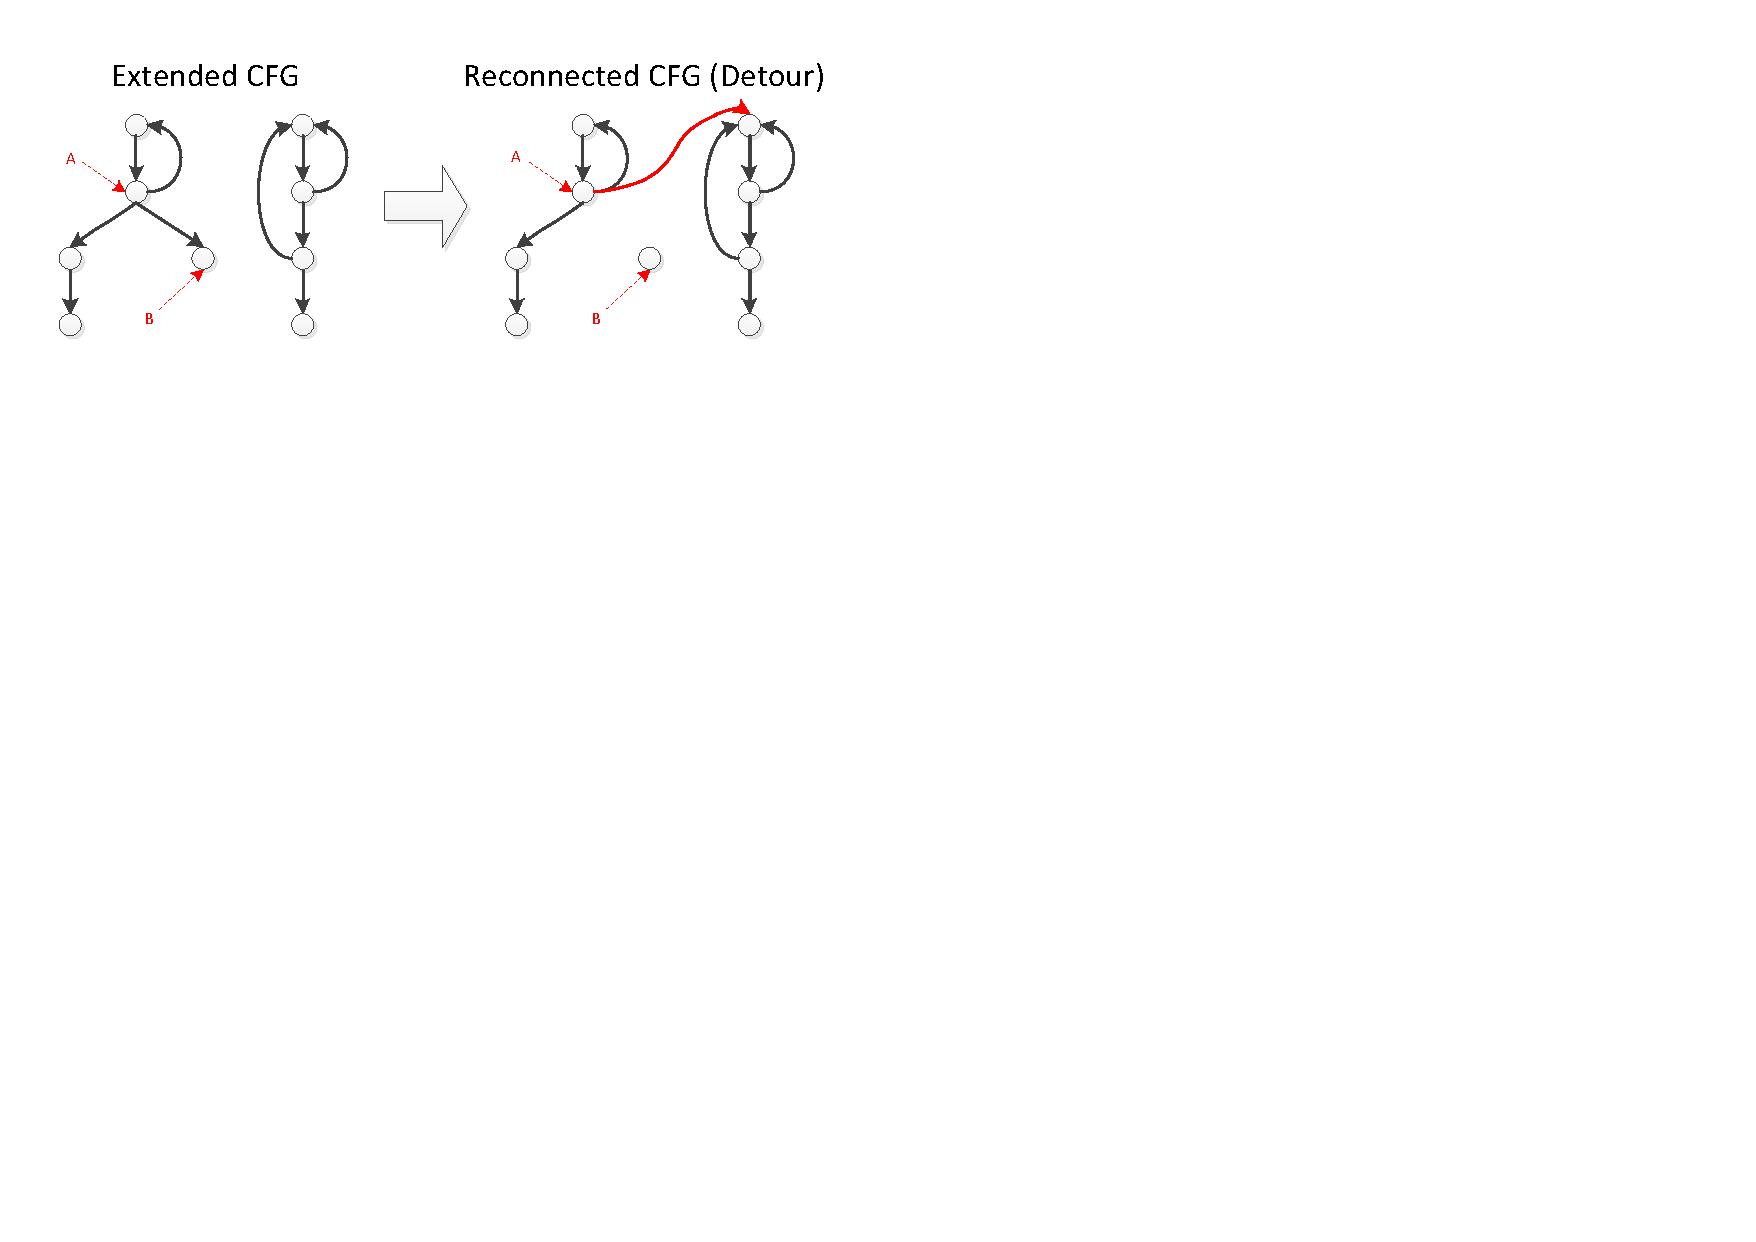
\includegraphics{Static_Patcher_Detour.pdf}
 \caption[Static Patcher Detour]{The static patcher adds, removes or modifies \emph{edges} of a CFG. This is the most basic case in which a single edge has been added to detour the execution of one basic block to another.}
\end{figure}

the role of the static patcher is to take a binary which is assumed to have all necessary code and 

IMPLEMENTATION
disasm engine builds on top of several abstractions. detailed diagram of disasm engine and how it works above libbfd and libopcodes. perhaps some justification for why we chose to use these

in practice, the disassembler engine is responsible for parsing and translating the strings received from libopcodes and storing that information in its internal semantic representation (bf\_insn, bf\_basic\_blk). bf\_func can be identified from three ways only:
1) if it is the target of a call site
2) if it corresponds to an address identified as a bf\_sym
3) if the user defined it as a root for cfg generation and explicitly stated it is a function (cfg analysis and generation is covered in depth in...)

further information such as size of symbols (which tells us size of function) is available because we are parsing the symbol table directly from libelf.

quirks of libopcodes disassembler such as how it passes us the instruction parts (mnemonic, operands, separator) as strings! we build a finite state machine which allows us to 

we can draw finite state machine in diagram here

binary\_file

within a binary\_file, there are 2 levels of code representation. firstly we have bf\_basic\_blk which represents a basic\_block as defined in architecture.

binary\_file is composed of a CFG of bf\_basic\_blk objects. during the process of cfg generation and after it completes, we add extra information. i.e., bf\_func 'labels'

bf\_func

implementation of CFG analysis and generation...

distribution and documentation

automake which we use to deal with library dependencies (libelf, libbfd, libopcodes, libkern).

 and doxygen

WORKFLOW



TESTING

we want to test robustness and reliability of the library. several areas in particular:

- we want make sure the library is scalable and does not fail on large scale systems. we test on real-world systems, as opposed to toy examples. namely, we test against coreutils (includes stuff like ls, cp, rm, etc.).

we have a suite of regression tests which test the following:

test 1: coreutils\_test32/64

so firstly we want to test the successful disassembly and cfg generation for some real-world example. 

probably want to use valgrind to check for errors